\chapter{Analisi dei requisiti}
\label{cap:analisi-requisiti}

\intro{In questa sezione vengono analizzati i requisiti del progetto e ne viene data un'analisi ad alto livello, combinando una visione concettuale con una visione pratica ed implementativa. 
Vengono inoltre descritti i casi d'uso e i requisiti individuati, con l'obiettivo di fornire una visione generale del sistema e delle sue funzionalità, in modo semplice e comprensibile.}

\section{Descrizione ed analisi del sistema}
L'obiettivo del progetto è la creazione di una piattaforma per la visualizzazione di contenuti multimediali, in questo caso dei film,
tramite l'utilizzo degli standard \glsfirstoccur{\gls{w3cg}} \glsfirstoccur{\gls{didg}} e \glsfirstoccur{\gls{ssig}} per la verifica sicura dell'identità dell'utente e per la 
visualizzazione di tutti i contenuti della piattaforma, certificando in modo sicuro la propria identità senza diffondere dati personali tramite 
l'utilizzo di un \glsfirstoccur{\gls{zkpg}}.\\

Più precisamente, l'implementazione avviene usando lo \textit{smart contract} che implementa ad alto livello lo standard \glsfirstoccur{\gls{ssig}}, 
scritto nel linguaggio di programmazione \textit{Solidity} da parte dello studente magistrale Alessio De Biasi.
Questo contratto permette la gestione dell'identità digitale tramite la creazione di un documento di identità digitale, che contiene un identificatore univoco
chiamato \glsfirstoccur{\gls{didg}}, composto da una stringa alfanumerica che identifica l'utente, e un \textit{DID Document}, che contiene le informazioni dell'utente a lui associato.
Normalmente, la sua creazione avviene tramite un file \textit{json}, composto dallo standard di riferimento, l'identificativo ed un campo \textit{controller},
che ha la capacità di fare dei cambiamenti al documento stesso e certifica la firma digitale del documento, sulla base del metodo usato per la sua creazione.
Il formato del \textit{DID Document} è come il seguente (codice proveniente da \cite{site:didw3c}):

\begin{lstlisting}[language=json]
    {
      "@context": [
        "https://www.w3.org/ns/did/v1",
        "https://w3id.org/security/suites/ed25519-2020/v1"
      ]
      "id": "did:example:123456789abcdefghi",
      "authentication": [{    
        "id": "did:example:123456789abcdefghi#keys-1",
        "type": "Ed25519VerificationKey2020",
        "controller": "did:example:123456789abcdefghi",
        "publicKeyMultibase": "zH3C2AVvLMv6gmMNam3uVAjZpfkcJCwDwnZn6z3wXmqPV"
      }]
    }
\end{lstlisting}

\newpage

Nel codice che dovrà essere utilizzato come libreria,
ogni documento è caratterizzato da una \textit{capability delegation}, che permette di delegare l'accesso crittografico di un elemento ad un altro utente,
un servizio, specificando l'identificativo e l'indirizzo di un'entità autorizzata, un metodo di autenticazione, in cui viene stabilito
il modo in cui implementare il meccanismo di riconoscimento da parte dell'utente (dimostrando di fatto che sia chi dice di essere) e un 
genitore, composto da un identificativo ed una firma digitale.
L'idea del codice è di creare una cosiddetta `catena di fiducia', la cui idea è associare ad un utente un \glsfirstoccur{\gls{didg}} e dimostrare,
attraverso un meccanismo di autenticazione definito a priori nel documento tramite firme digitali, la risoluzione dei dati trasmessi, il riconoscimento univoco della sua identità
e l'accesso ad un determinato contenuto. Infatti, l'utente viene riconosciuto perché i suoi dati sono stati certificati da un ente 
con capacità di firma digitale che, a sua volta, si fida di altri enti anch'essi riconosciuti, fino ad arrivare ad un soggetto radice.
Se questa catena di fiducia viene risolta correttamente, l'utente viene riconosciuto univocamente e può accedere ai contenuti della piattaforma. \\

La struttura dati blockchain, attraverso l'utilizzo di un account associato ad un \glsfirstoccur{\gls{didg}}, permette di certificare l'identità dell'utente
tramite la firma digitale dei dati trasmessi con la propria coppia di chiavi pubblica/privata, certificando in modo immutabile la propria identità e
permette di realizzare un sistema di autenticazione sicuro e decentralizzato, che non richiede l'utilizzo di un ente terzo per la verifica delle informazioni. \\

L'utilizzo della piattaforma e delle sue parti prescinde dalla dimostrazione, attraverso una chiamata al contratto libreria fornito, della risoluzione attraverso firma digitale
del \glsfirstoccur{\gls{didg}} associato all'utente, che dimostra l'utilizzo di un account associato alla rete blockchain,
la sua identità. Se l'indirizzo che ha firmato digitalmente il documento è associato ad un profilo creatore di quel \glsfirstoccur{\gls{didg}} così firmato,
allora l'utente può accedere ai contenuti della piattaforma. L'implementazione di questo passaggio prevede che l'utente dimostri precisamente
la propria identità secondo un meccanismo \textit{challenge-response}: viene generato un numero casuale e viene chiesto all'utente di firmarlo digitalmente, in modo da dimostrare
che è in possesso della chiave privata associata all'indirizzo che ha firmato il documento. \\

Se il metodo di autenticazione conteneva la sua firma e come dato il numero casuale trasmesso, grazie alla generazione dell'identificatore
e la chiamata al contratto in grado di risalire precisamente all'account blockchain che l'ha emessa, si certifica l'utente in modo univoco.
Tale meccanismo viene implementato in fase di registrazione, in cui l'utente possiede un proprio \glsfirstoccur{\gls{didg}} e registra i propri dati anagrafici
e in fase di accesso, quando l'utente inserita esclusivamente come unico dato per effettuare il login il proprio identificatore, firmato digitalmente nella fase precedente e appartenente in modo univoco a lui. \\

In questa sezione, l'utente viene presentato ad un insieme di film e può scegliere di visualizzarne uno. Alla visualizzazione di un certo
contenuto oggetto a limiti di età, l'utente viene presentato ad una schermata di verifica, in cui deve dimostrare la sua età.
Questo passaggio avviene attraverso la creazione di una \glsfirstoccur{\gls{vpg}}, contenente molteplici \glsfirstoccur{\gls{vcg}}, 
con una associata all'utente (definito \textit{holder} delle credenziali) e le altre associate agli enti verificatori (definiti \textit{issuer}, che sono gli enti che hanno rilasciato le credenziali). \\

Normalmente, una \textit{Verifiable Presentation} è infatti composta da:
\begin{itemize}
    \item un insieme di metadati, che descrivono la presentazione;
    \item un insieme di \textit{Verifiable Credentials}, che sono le credenziali associate alla presentazione;
    \item un insieme di \textit{proof}, che sono le prove di autenticità delle credenziali.
\end{itemize}

Invece, una \textit{Verifiable Credential} è composta da:
\begin{itemize}
    \item un contesto di riferimento, che è un \textit{URI} che definisce il contesto di riferimento delle credenziali;
    \item un identificativo, che specifica il sito di riferimento;
    \item un tipo, che specifica se la credenziale è appropriata per la presentazione;
    \item un soggetto, che è l'identificativo dell'utente a cui sono associate le credenziali;
    \item un \textit{issuer}, che è l'identificativo dell'ente che ha rilasciato le credenziali;
    \item un \textit{issuanceDate}, che è la data di rilascio delle credenziali;
    \item una \textit{proof}, che è la prova di autenticità delle credenziali.
\end{itemize}

Il seguente è un esempio di una \textit{Verifiable Presentation} con al suo interno un insieme di \textit{Verifiable Credentials} (codice proveniente da \cite{site:vpw3c}):
\begin{lstlisting}[language=json]
    {
        "@context": [
          "https://www.w3.org/2018/credentials/v1",
          "https://www.w3.org/2018/credentials/examples/v1"
        ],
        "type": "VerifiablePresentation",
        "verifiableCredential": [
          {
            "@context": [
              "https://www.w3.org/2018/credentials/v1",
              "https://www.w3.org/2018/credentials/examples/v1"
            ],
            "type": ["VerifiableCredential", "UniversityDegreeCredential"],
            "credentialSchema": {
              "id": "did:example:cdf:35LB7w9ueWbagPL94T9bMLtyXDj9pX5o",
              "type": "did:example:schema:22KpkXgecryx9k7N6XN1QoN3gXwBkSU8SfyyYQG"
            },
            "issuer": "did:example:Wz4eUg7SetGfaUVCn8U9d62oDYrUJLuUtcy619",
            "credentialSubject": {
              "degreeType": "BachelorDegree",
              "degreeSchool": "College of Engineering"
            },
            "proof": {
              "type": "AnonCredDerivedCredentialv1",
              "primaryProof": "cg7wLNSi48K5qNyAVMwdYqVHSMv1Ur8i...Fg2ZvWF6zGvcSAsym2sgSk737",
              "nonRevocationProof": "mu6fg24MfJPU1HvSXsf3ybzKARib4WxG...RSce53M6UwQCxYshCuS3d2h"
            }
        }],
        "proof": {
          "type": "AnonCredPresentationProofv1",
          "proofValue": "DgYdYMUYHURJLD7xdnWRinqWCEY5u5fK...j915Lt3hMzLHoPiPQ9sSVfRrs1D"
        }
      }
\end{lstlisting}

Al suo interno, come si vede, sono presenti un insieme di credenziali, contenente un campo di dimostrazione di appartenenza ad uno schema comune,
a cui sarà associata la catena di fiducia, e degli insiemi di metodi di firma digitale, che dimostrano la validità delle credenziali presenti,
avendo ciascuna un insieme di \textit{issuer} riconosciuti. \\

Il meccanismo è in grado di integrarsi con \glsfirstoccur{\gls{zkpg}}, in cui la prova di appartenenza ad uno schema comune è dimostrata
senza rivelare informazioni sensibili di alcun tipo, combinando un insieme di \textit{Verifiable Credentials}, verificate tramite 
un insieme di \textit{issuer} riconosciuti dal sistema della catena di fiducia grazie all'uso della proprietà \textit{proof} descritta sopra
e la definizione di uno schema comune a cui fare riferimento, che certifica il riconoscimento in quanto firmato a catena da un insieme di \textit{issuer}
(secondo le specifiche dettagliate in \cite{site:zkpw3c}). \\
Questo permette all'utente di definire precisamente quali informazioni vuole rivelare e, attraverso l'utilizzo del contratto libreria, 
dimostrare la propria identità, verificato con questo meccanismo e accedendo al proprio contenuto di interesse. 

\section{Casi d'uso}

In questa sezione, saranno presenti un insieme di diagrammi dei casi d'uso, definiti secondo il linguaggio standard \glsfirstoccur{\gls{umlg}},
che descrivono le interazioni tra gli attori, definiti convenzionalmente come utenti del sistema e il sistema stesso. 
Seguirà una tabella di tracciamento dei requisiti, che mostrerà come i requisiti individuati nella sezione precedente siano soddisfatti
dai casi d'uso definiti in questa sezione, in base all'analisi prevista. \\
\\

%\begin{figure}[!h] 
%    \centering 
%    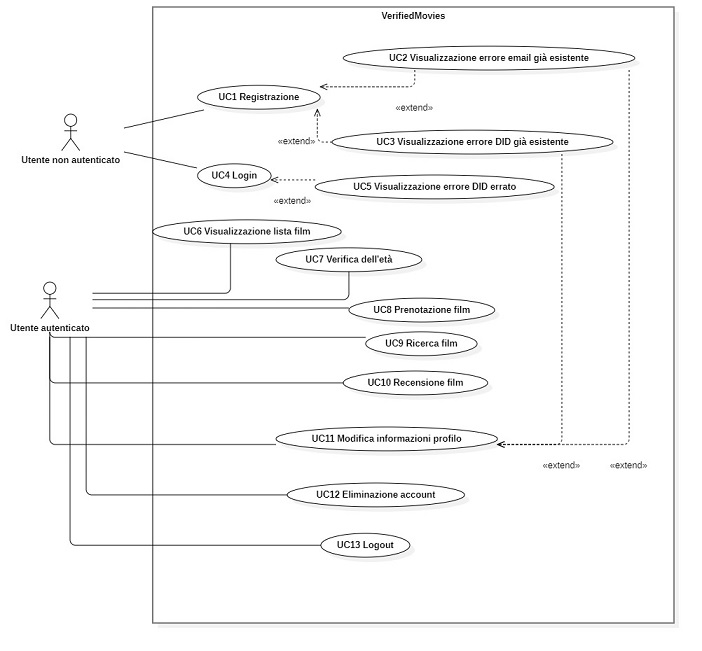
\includegraphics[width=0.9\columnwidth]{usecase/scenario-principale} 
%    \caption{Use Case - UC0: Scenario principale}
%\end{figure}
%
%\begin{usecase}{0}{Scenario principale}
%\usecaseactors{Sviluppatore applicativi}
%\usecasepre{Lo sviluppatore è entrato nel plug-in di simulazione all'interno dell'IDE}
%\usecasedesc{La finestra di simulazione mette a disposizione i comandi per configurare, registrare o eseguire un test}
%\usecasepost{Il sistema è pronto per permettere una nuova interazione}
%\label{uc:scenario-principale}
%\end{usecase}
%
%\section{Tracciamento dei requisiti}
%
%Da un'attenta analisi dei requisiti e degli use case effettuata sul progetto è stata stilata la tabella che traccia i requisiti in rapporto agli use case.\\
%Sono stati individuati diversi tipi di requisiti e si è quindi fatto utilizzo di un codice identificativo per distinguerli.\\
%Il codice dei requisiti è così strutturato R(F/Q/V)(N/D/O) dove:
%\begin{enumerate}
%	\item[R =] requisito
%    \item[F =] funzionale
%    \item[Q =] qualitativo
%    \item[V =] di vincolo
%    \item[N =] obbligatorio (necessario)
%    \item[D =] desiderabile
%    \item[Z =] opzionale
%\end{enumerate}
%Nelle tabelle \ref{tab:requisiti-funzionali}, \ref{tab:requisiti-qualitativi} e \ref{tab:requisiti-vincolo} sono riassunti i requisiti e il loro tracciamento con gli use case delineati in fase di analisi.
%
%\newpage
%
%\begin{table}%
%\caption{Tabella del tracciamento dei requisiti funzionali}
%\label{tab:requisiti-funzionali}
%\begin{tabularx}{\textwidth}{lXl}
%\hline\hline
%\textbf{Requisito} & \textbf{Descrizione} & \textbf{Use Case}\\
%\hline
%RFN-1     & L'interfaccia permette di configurare il tipo di sonde del test & UC1 \\
%\hline
%\end{tabularx}
%\end{table}%
%
%\begin{table}%
%\caption{Tabella del tracciamento dei requisiti qualitativi}
%\label{tab:requisiti-qualitativi}
%\begin{tabularx}{\textwidth}{lXl}
%\hline\hline
%\textbf{Requisito} & \textbf{Descrizione} & \textbf{Use Case}\\
%\hline
%RQD-1    & Le prestazioni del simulatore hardware deve garantire la giusta esecuzione dei test e non la generazione di falsi negativi & - \\
%\hline
%\end{tabularx}
%\end{table}%
%
%\begin{table}%
%\caption{Tabella del tracciamento dei requisiti di vincolo}
%\label{tab:requisiti-vincolo}
%\begin{tabularx}{\textwidth}{lXl}
%\hline\hline
%\textbf{Requisito} & \textbf{Descrizione} & \textbf{Use Case}\\
%\hline
%RVO-1    & La libreria per l'esecuzione dei test automatici deve essere riutilizzabile & - \\
%\hline
%\end{tabularx}
%\end{table}%
